% !TeX root = ../thuthesis-example.tex

\chapter{引言}

\section{研究背景及意义}
\subsection{背景概述}
数字人技术的发展历程经历了从平面影像合成向三维空间交互的范式迁移。早期数字人主要以二维（2D）形态为主，基于图像序列合成、生成对抗网络（GAN）\cite{goodfellow2020generative}等技术，实现了较高保真度的视觉复现。尽管 2D 数字人在表情驱动和谈话头部（Talking Head）等局部交互场景中表现出色，但其角色形象通常高度同质化，且受限于平面维度的本质，在空间位移、多视角观察以及复杂肢体协同方面存在天然瓶颈，难以支撑具有强个性表达与高动态要求的艺术表现。随着虚拟现实（VR）、增强现实（AR）以及计算机图形学的跨代式发展，数字人技术逐步突破维度限制，迈向三维（3D）具身化阶段。相较于 2D 技术，3D 数字人不仅依托完整的空间几何结构与复杂的骨骼运动学链实现全身动态展示，同时也为角色外观的精细建模与个性化编辑提供了更大的设计自由度，使数字人在形体比例、风格特征等方面具备更强的可塑性。尤其在电影特效、高沉浸感游戏及虚拟直播等领域，三维数字人已成为推动用户体验创新的重要载体。

当前数字人的研究正从以静态外观拟真，逐步演进为对角色外观个性与动态行为建模的综合阶段。一方面，角色外表的个性化编辑通过对面部特征、体型结构、服饰风格与整体美学气质的设计，直接决定了数字人的视觉辨识度与情感投射能力，是构建角色人格与身份认同的基础；另一方面，角色动作，尤其是全身动作的生成，则进一步塑造了其行为风格与情绪表达的连续性。其中，全身动作生成技术构成了高表现力数字人的核心技术支撑。传统的动作捕捉或动作重定向方法多侧重于运动轨迹的物理复刻，往往忽略动作风格与角色外观、性格之间的内在关联，难以充分刻画动作中所蕴含的情绪张力。因此，如何在保持动作物理合理性的同时，使生成结果在风格上与角色外观特征保持一致，并具备对情感意图的表达能力，已成为计算机视觉和计算机图形学交叉领域的重要研究方向。

舞蹈作为一种古老而独特的艺术形态，是人类情感表达与思想传达的高级范式之一。通过高度协调且富有节奏感的身体运动，舞蹈能够突破语言的限制与文化的隔阂，构建起跨群体的情感沟通桥梁。舞蹈的表现力源于其复杂而精细的身体动作语言，而这种表现力往往与舞者的形体特征及舞台形象密切相关。对于 3D 数字人而言，舞蹈动作生成并非简单的物理位移计算，而是与角色外观风格相互耦合的情感表达过程，需要在视觉形象与动作语义之间建立一致性。因此，研究高表现力的舞蹈动作生成，不仅是图形学领域追求视觉真实的必然延伸，更是实现数字人在形象风格—动作表达层面高度统一的重要途径。

随着三维数字人技术逐步渗透至社会生活的各个层面，市场与应用场景对三维数字人表现力的需求持续提升。三维数字人的角色定位已从早期的基础交互工具（如聊天机器人、辅助性虚拟角色），演变为具备高度社会属性的虚拟偶像、娱乐形象及情感陪伴者。在这一过程中，角色外观的差异化设计与可持续编辑能力，成为三维数字人建立长期用户认同的重要前提。同时，这一转变也对三维数字人在情感交流与深度互动提出了更为严苛的要求。在现实应用中，三维数字人不仅需要稳定的视觉呈现，更需要在与其外观形象相匹配的行为与动作层面，展现出足够的细腻度与情感丰富性。尤其在虚拟偶像演出、虚拟直播及沉浸式社交场景中，角色外观个性化与全身舞蹈动作生成需求呈现出快速增长趋势。通过富有艺术感染力的舞蹈动作，三维数字人能够更完整地传递其角色设定与情感内涵，显著增强用户的沉浸感与心理认同。因此，探索同时支持角色外观个性化编辑与高表现力三维数字人全身舞蹈动作生成的技术框架，对于构建更具生命感与情感连接的数字交互空间，具有重要的学术价值与现实意义。

\subsection{研究意义}
舞蹈动作生成作为数字人动作生成技术的一项重要任务，具备独特的挑战与价值。传统的动作生成方法通常侧重于基础动作的模仿和重现，而舞蹈动作生成则需要在空间、节奏、情感等方面进行更深层次的理解~\cite{fink2021evolution, kico2018digitization}。舞蹈不仅仅是身体的移动，它更是情感的传达和个性的体现。因此，如何通过技术手段生成具有表现力和情感共鸣的舞蹈动作，成为当前数字人技术发展的重要课题。在数字人情感表达方面，舞蹈能够有效地拉近数字人与用户之间的情感距离，使用户感受到更加生动和具有深度的互动体验。数字人通过舞蹈动作的生成，不仅可以展现情感的变化，还能够在娱乐、教育、社交等领域中提供更加沉浸和富有表现力的内容体验。

通常数字人舞蹈动作的编排通常依赖于人工设计或基于传统的动画方法。这种方式不仅费时且劳动强度大，还对编排者的艺术感知和创作能力提出了较高的要求。尤其是当需要为数字人生成大量具有高表现力和情感丰富度的舞蹈动作时，人工编排往往面临效率低、创造力受限等问题。因此，自动化数字人舞蹈动作生成技术的研究具有重要意义。通过借助人工智能和深度学习技术，自动化生成舞蹈动作不仅能够大幅度提升工作效率，还能降低人力成本。更为重要的是，借助先进的舞蹈生成算法，能够根据角色的情感需求和动作风格，生成更加多样化且具有高表现力的舞蹈动作，从而拓宽数字人动作生成的创作空间。舞蹈生成技术的应用还能够将复杂动作的编排过程简化，对于大规模虚拟人物的内容生产具有显著的推动作用。

% \begin{figure}[b]
%   \centering
%   \includegraphics[width=0.8\linewidth]{figures/DateToParameter.png}
%   \caption{1954年至2021年间流行的机器学习模型规模（parameters）与发布时间（publication date）变化关系图\cite{datetoparameters}。}
%   \label{fig:DateToParameter}
% \end{figure}

\subsection{问题与挑战}

三维数字人的高表现力的挑战主要体现在外观与动作两个层面。在外观层面，如何在保证结构一致性与生成效率的前提下，实现高效、灵活且可控的个性化编辑，仍面临模型表达能力受限、编辑稳定性不足等挑战。在动作层面，高表现力舞蹈生成需要同时满足动作的真实感、整体协调性以及与音乐等条件的精确对齐，但现有方法在高质量数据获取、长时序建模以及全身动作一致性方面仍存在明显不足。主要技术路线和应用价值如图~\ref{fig:tech_path}。这些问题共同制约了高表现力三维数字人的生成效果与实际应用。


\subsubsection{外观个性化编辑的挑战} 在外观层面，高表现力数字人需要支持高效且灵活的个性化编辑，以满足不同用户在身份特征、审美风格和应用场景上的多样化需求。具体而言，数字人外观不仅应在整体形象上具备良好的辨识度，还应支持对发型、服饰、体型比例以及面部细节等多维外观属性的精细化控制。同时，外观编辑过程应具备较高的效率与易用性，避免依赖大规模个体数据或复杂的模型重训练，从而降低个性化建模的成本并提升实际应用中的可扩展性。这对外观表示的解耦性、可控性以及生成模型的编辑能力均提出了更高要求。

\noindent\textbf{基于参数化模型的个性化外观生成}\quad 基于参数化模型的个性化外观生成方法通过一组可解释的形状、姿态和表情参数对三维数字人的外观进行建模，在结构一致性与物理合理性方面具有一定优势。然而，该类方法在实现高表现力与高度个性化外观表达时仍存在明显局限。首先，参数化模型通常依赖低维参数空间刻画复杂的人体或面部形态，其表达能力受模型先验约束，难以准确表示个体层面的高频几何细节与精细外观特征，如面部微表情、肌肉起伏及服饰细节等，从而影响视觉真实感。其次，模型的形状与外观空间通常由特定数据分布学习得到，当目标个体特征超出该分布范围时，容易产生过度平滑或形态失真的问题，限制个性化建模的灵活性。最后，在动态场景下，形状、姿态与表情参数之间的耦合关系可能导致外观随动作变化出现不稳定或不自然的现象。

\noindent\textbf{基于模型微调的个性化外观生成}\quad 基于模型微调的个性化外观生成方法通常通过对预训练生成模型进行再训练，使模型参数显式地适配特定个体外观特征，从而实现较高程度的个性化表达。然而，该类方法在实际应用中仍面临多方面挑战。首先，模型微调往往依赖一定规模的个体数据，数据采集与标注成本较高，限制了方法在大规模个性化场景中的适用性。其次，针对单一或少数个体进行微调容易导致模型过拟合，使其泛化能力下降，在面对不同姿态、光照或外观变化时稳定性不足。此外，模型微调过程通常计算开销较大，训练时间较长，对硬件资源和工程实现提出了较高要求，不利于快速迭代和实时应用。与此同时，频繁的模型参数更新也可能破坏原有模型在其他任务或风格上的生成能力，引发灾难性遗忘问题。最后，在多身份或多风格共存的应用场景中，如何在保证个性化效果的同时实现不同个体之间的有效区分与统一管理，仍是基于模型微调方法亟待解决的关键问题。

\noindent\textbf{基于注意力机制的个性化外观生成}\quad 基于注意力机制的个性化外观生成方法通过在生成过程中引入自注意力或交叉注意力结构，实现对特定身份特征或外观区域的精细化控制，在无需或仅需少量训练的条件下展现出较强的编辑灵活性。然而，现有方法在个性化外观编辑的效率与稳定性方面仍面临诸多挑战。首先，部分方法依赖 DDIM~\cite{song2020denoising} 反演过程将图像映射至扩散模型的隐空间，该过程通常需要较长的迭代步数，且容易导致中间隐变量偏离原始生成轨迹，从而影响重建质量，限制编辑效果的可靠性~\cite{mokady2022null}。其次，基于文本提示的注意力控制方式受到自然语言歧义性和表达不精确性的影响，用户意图与生成结果之间往往存在较大偏差，且在多数文本到图像模型中，提示词的微小变化也可能引发生成结果的显著差异，降低了编辑过程的可控性与一致性~\cite{cao2023masactrl}。此外，现有基于注意力机制的方法大多局限于二维图像空间，缺乏对视频序列和三维场景等更复杂视觉表示的有效支持~\cite{hertz2022prompt}，限制了其在动态内容生成与三维数字人建模等高表现力应用场景中的进一步拓展。

\begin{figure}[h]
  \centering
  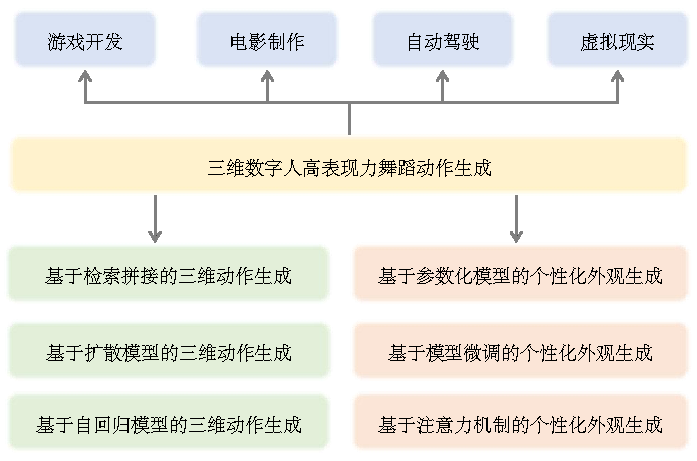
\includegraphics[width=0.8\linewidth]{figures/tech_path.pdf}
  \caption{三维数字人高表现力舞蹈动作生成技术及应用场景}
  \label{fig:tech_path}
\end{figure}

\subsubsection{高表现力舞蹈动作生成的挑战}
三维数字人动作高表现力主要体现在舞蹈动作生成的真实感、全身关节的协调性以及与音乐条件在节奏与情绪层面的契合程度。而现有的三维数字人舞蹈动作生成方法仍面临多方面挑战：首先，高质量舞蹈数据集较为稀缺，现有数据多依赖姿态估计方法从视频或多视角图像中重建三维动作，易引入估计误差，且通常缺乏对手势动作与面部表情的完整建模；其次，生成的舞蹈动作与输入音乐在节奏结构和情绪表达上的对齐性不足，难以充分体现“闻歌起舞”的艺术特征；此外，现有方法往往仅关注身体主体动作，缺少对全身动作（包括手部与面部）的统一建模，导致整体舞蹈表现缺乏协调性与感染力。

除此之外，现有数字人动作生成方法在建模范式与应用侧重点上呈现出明显差异，其优缺点对比如表~\ref{tab:2d_vs_3d} 所示。2D 动作生成在生产效率方面具有优势，但动作自由度和真实感有限；基于检索拼接的 3D 方法在动作时长和稳定性上表现较好，但交互能力不足；自回归与扩散模型的 3D 动作生成在动作自由度、真实感和交互能力方面更具潜力。

\begin{table}
    \caption{二维与三维数字人动作生成技术方案优缺点对比}
    \label{tab:2d_vs_3d} 
    \centering
    \resizebox{\linewidth}{!}{
        \begin{tabular}{lccccc}
            \toprule [1pt]
            技术方案
            & 生产效率 & 动作自由度 & 视觉真实感 & 动作时长 & 交互能力 \\
            \noalign{\smallskip}\midrule[0.5pt]
            \noalign{\smallskip}
            二维动作生成 & \ding{72}\ding{72}\ding{72}\ding{72} & \ding{72} & \ding{72}\ding{72}  & \ding{72}\ding{72} &\ding{72}\\
            基于检索拼接的三维动作生成 & \ding{72}\ding{72}\ding{72} & \ding{72}\ding{72} & \ding{72}\ding{72}  &\ding{72}\ding{72}\ding{72} &\ding{72}\\
            基于自回归模型的三维动作生成 & \ding{72}\ding{72}\ding{72}\ding{72} & \ding{72}\ding{72}\ding{72}\ding{72} & \ding{72}\ding{72}\ding{72}  & \ding{72}\ding{72}\ding{72}\ding{72} & \ding{72}\ding{72}\ding{72}\\
            基于扩散模型的三维动作生成  & \ding{72}\ding{72} & \ding{72}\ding{72}\ding{72}\ding{72} & \ding{72}\ding{72}\ding{72}\ding{72}  &\ding{72} &\ding{72}\ding{72}\ding{72}\\
            \bottomrule [1pt] 
            %\noalign{\smallskip}
        \end{tabular}
        }

\end{table}


\noindent\textbf{基于检索拼接的三维动作生成}\quad 基于拼接检索的 3D 动作生成方法通过从动作数据库中检索与当前条件最相似的动作片段并进行拼接，以实现较为自然的运动合成，在一定程度上能够保证动作的真实性和物理合理性~\cite{arikan2002interactive, kim2003rhythmic, shiratori2006dancing, tang2018dance, au2022choreograph}。然而，该类方法在高表现力动作生成任务中仍存在明显局限。首先，其生成效果高度依赖于动作库的规模与多样性，当数据库覆盖不足时，容易出现动作重复或表现单一的问题，限制生成结果的丰富性。其次，不同动作片段之间在时序连续性和语义一致性方面难以保证，简单拼接往往导致动作衔接不自然，整体协调性不足。此外，该类方法缺乏对高层语义条件（如音乐节奏、情绪变化等）的建模能力，难以实现与输入条件的精细对齐，从而限制了其在复杂舞蹈生成场景中的应用。

\noindent\textbf{基于扩散模型的三维动作生成}\quad 基于扩散模型的 3D 动作生成方法通过逐步去噪的方式建模复杂动作分布，在生成多样性和稳定性方面展现出显著优势，近年来已成为三维动作生成领域的重要研究方向。然而，该类方法在高表现力 3D 动作生成任务中仍面临多方面挑战。首先，扩散模型通常依赖较长的采样过程，推理阶段需要多步迭代去噪，导致生成效率较低，难以满足实时或交互式应用需求。其次，动作数据本身具有高维、强时序相关性的特点，如何在扩散过程中有效建模长时序依赖关系，并保持动作在时间维度上的连贯性与物理合理性，仍是一个具有挑战性的问题。此外，在条件生成场景下，将音乐节奏、情绪或语义信息等外部条件与动作生成过程进行精确对齐仍然较为困难，容易出现动作与条件响应不充分或不一致的情况。最后，扩散模型对大规模高质量训练数据具有较强依赖，而包含精细手势与面部表情的完整 3D 动作数据较为稀缺，这在一定程度上限制了模型在高表现力舞蹈生成等复杂应用场景中的进一步发展。

\noindent\textbf{基于自回归模型的三维动作生成}\quad 基于自回归模型的 3D 动作生成方法通过对动作序列进行逐帧或逐时间步建模，显式刻画动作在时间维度上的演化过程，在时序建模与条件控制方面具有一定优势~\cite{siyao2022bailando,li2021ai}。然而，该类方法在高表现力 3D 动作生成任务中仍面临多方面挑战。首先，自回归生成过程依赖前序预测结果，误差在时间维度上容易不断累积，从而导致长序列动作出现漂移、抖动或不自然的问题，影响整体动作质量。其次，逐步生成的方式限制了模型对全局时序结构的感知能力，难以同时兼顾局部动作细节与整体节奏变化，进而影响舞蹈动作的连贯性与表现力。此外，自回归模型在推理阶段通常需要顺序生成，难以并行计算，导致生成效率较低，不利于大规模或实时应用场景。与此同时，在复杂条件驱动的任务中，将音乐节奏、情绪语义等高层条件有效融入自回归框架仍具有一定难度，容易出现条件响应不充分的问题。最后，该类方法对高质量长时序动作数据具有较强依赖，而此类数据的获取成本较高，进一步限制了模型性能的提升与实际应用。


% \subsection{研究动机}

% \section{研究意义}

% \subsection{游戏开发领域}

% \subsection{虚拟现实领域}

% \subsection{电影制作领域}


\section{研究思路和目标}
本研究围绕“高表现力三维数字人舞蹈内容生成”这一核心目标展开，如图~\ref{fig:research_struct}所示，聚焦数字人舞蹈在外观个性化表达与动作生成质量两个关键维度上的协同建模问题，探索一种能够在无需额外训练或弱训练条件下，实现角色外观可控编辑与音乐对齐舞蹈动作联合生成的统一技术框架。

从整体思路上看，本研究以“分层建模、模块解耦、跨模态对齐”为基本原则：在视觉层面，通过外观个性化编辑增强数字人角色的身份区分度与表现张力；在动作层面，通过音乐驱动的全身舞蹈动作生成，提升数字人在时序一致性、动作协调性及情绪表达上的综合表现；并在此基础上，引入分层级联的动作建模与音乐对齐机制，实现外观与动作之间的语义一致与风格统一。整体研究框架如图所示，涵盖外观个性化编辑、舞蹈动作生成以及综合研究目标三个层面。

\begin{figure}[h]
  \centering
  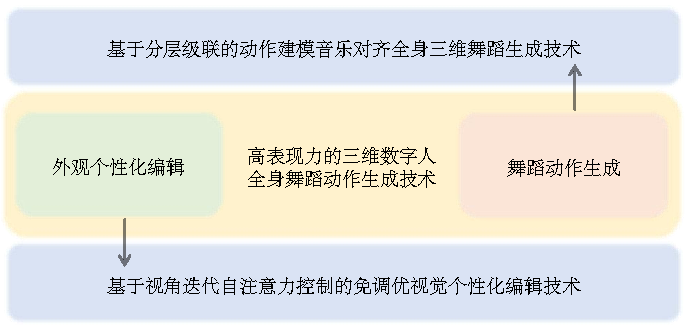
\includegraphics[width=0.9\linewidth]{figures/research_struct.pdf}
  \caption{研究思路结构图}
  \label{fig:research_struct}
\end{figure}

\subsection{角色外观生成}
数字人外观是其身份认知与情感传达的重要载体。传统数字人舞蹈生成方法通常假设角色外观固定，或仅通过简单的贴图替换、参数化建模等方式进行外观调整，难以在保持角色结构一致性的同时，实现多视角、多部位协调的个性化编辑。此外，现有基于扩散模型或生成对抗网络的视觉编辑方法，多依赖额外微调或局部重训练，存在计算成本高、泛化能力有限等问题，难以满足高效、灵活的数字人创作需求。

针对上述问题，本研究从无需训练（training-free）视觉编辑的角度出发，探索一种基于视角迭代自注意力控制机制的数字人外观个性化编辑方法。该方法通过在扩散过程中的多步迭代中，引入跨视角一致性的自注意力约束，在不引入额外参数学习的前提下，实现对数字人局部外观属性（如服饰、颜色、材质风格等）的精细化控制。同时，该机制能够有效抑制多视角生成中常见的外观漂移与结构失真问题，保证编辑结果在不同视角下的空间一致性与语义稳定性。

通过该外观个性化编辑模块，本研究旨在为后续舞蹈动作生成提供稳定且风格明确的角色视觉表达基础，使数字人在舞蹈过程中能够保持清晰一致的角色形象，从而提升整体舞蹈表现的沉浸感与辨识度。
\subsection{舞蹈动作生成}
在舞蹈动作层面，高表现力不仅体现在单帧姿态的自然性，更体现在长时序动作的连贯性、全身关节的协调性以及与音乐节奏和情绪的高度对齐。然而，现有音乐驱动的三维舞蹈生成方法多采用单层时序建模策略，难以同时兼顾全局结构与局部细节；同时，部分方法仅关注身体主体动作，对手部、脚步及身体重心变化建模不足，导致生成舞蹈在表现力与真实感上存在明显局限。

针对上述挑战，本研究提出一种基于分层级联的动作建模与音乐对齐的全身三维舞蹈生成思路。该思路通过将舞蹈动作分解为不同时间与空间尺度的子模块，在高层建模整体节奏与动作结构，在低层细化关节运动与局部表现，从而实现对舞蹈动作的层次化控制。同时，引入音乐特征驱动机制，在节拍、能量变化及情绪特征等多个维度上对动作生成过程进行约束，使生成舞蹈能够更好地体现“闻歌起舞”的艺术特性。通过分层动作建模与音乐对齐机制的结合，本研究力图在保证动作物理合理性的同时，显著提升舞蹈生成的表现力、丰富度与多样性，为高质量三维数字人舞蹈生成提供可靠的技术支撑。

\subsection{研究目标}
本研究围绕高表现力三维数字人的关键技术瓶颈，分别从外观个性化编辑与舞蹈动作生成两个核心方向开展研究，系统性提升三维数字人在视觉表达与动作表现方面的整体表现力，具体研究目标可概括为以下两个方面：

1. 提出一种高效、稳定的数字人外观个性化编辑方法，在无需额外训练或微调的条件下，实现多视角一致、结构稳定的视觉编辑效果。该目标旨在解决现有数字人外观编辑方法中普遍存在的视角不一致、结构漂移及泛化能力不足等问题，为高表现力数字人提供可控、可靠的角色外观表达能力。

2. 设计一种音乐对齐的分层级联舞蹈动作生成模型，在全身尺度上实现对舞蹈动作的协调建模与情绪表达。通过对舞蹈动作的层次化时序建模与音乐特征对齐，提升三维数字人舞蹈在节奏一致性、动作连贯性以及艺术表现力方面的整体质量。

通过在外观个性化编辑与舞蹈动作生成两个方向上的研究与技术突破，本研究致力于从不同维度增强三维数字人的表现能力，为高质量数字内容创作与虚拟人应用提供具有实践价值的技术支撑与研究思路。



\iffalse


\section{摘要的写法}

论文摘要是对论文研究内容的高度概括，应具有独立性和自含性，即应是 一篇简短但意义完整的文章。
通过阅读论文摘要，读者应该能够对论文的研究 方法及结论有一个整体性的了解，因此摘要的写法应力求精确简明。
论文摘要 应包括对问题及研究目的的描述、对使用的方法和研究过程进行的简要介绍、 对研究结论的高度凝练等，重点是结果和结论。

论文摘要切忌写成全文的提纲，尤其要避免“第 1 章……；第 2 章……；……”这样的陈述方式。



\section{引言的写法}

一篇学位论文的引言大致包含如下几个部分：
1、问题的提出；
2、选题背 景及意义；
3、文献综述；
4、研究方法；
5、论文结构安排。
\begin{itemize}
  \item 问题的提出：要清晰地阐述所要研究的问题“是什么”。
    \footnote{选题时切记要有“问题意识”，不要选不是问题的问题来研究。}
  \item 选题背景及意义：论述清楚为什么选择这个题目来研究，即阐述该研究对学科发展的贡献、对国计民生的理论与现实意义等。
  \item 文献综述：对本研究主题范围内的文献进行详尽的综合述评，“述”的同时一定要有“评”，指出现有研究状态，仍存在哪些尚待解决的问题，讲出自己的研究有哪些探索性内容。
  \item 研究方法：讲清论文所使用的学术研究方法。
  \item 论文结构安排：介绍本论文的写作结构安排。
\end{itemize}



\section{正文的写法}

本部分是论文作者的研究内容，不能将他人研究成果不加区分地掺和进来。
已经在引言的文献综述部分讲过的内容，这里不需要再重复。
各章之间要存在有机联系，符合逻辑顺序。



\section{结论的写法}

结论是对论文主要研究结果、论点的提炼与概括，应精炼、准确、完整，使读者看后能全面了解论文的意义、目的和工作内容。
结论是最终的、总体的结论，不是正文各章小结的简单重复。
结论应包括论文的核心观点，主要阐述作者的创造性工作及所取得的研究成果在本领域中的地位、作用和意义，交代研究工作的局限，提出未来工作的意见或建议。
同时，要严格区分自己取得的成果与指导教师及他人的学术成果。

在评价自己的研究工作成果时，要实事求是，除非有足够的证据表明自己的研究是“首次”、“领先”、“填补空白”的，否则应避免使用这些或类似词语。

\fi